%%%%%%%%%%%%%%%%%%%%%%%%%%
%%% Most used packages %%%
%%%%%%%%%%%%%%%%%%%%%%%%%%
\documentclass[a4paper]{memoir}
\usepackage[utf8]{inputenc}
\usepackage[T1]{fontenc}
\usepackage{hyperref}
\usepackage{amsmath}
\usepackage{amssymb}
\usepackage{amsthm}
\usepackage{stmaryrd}
\usepackage{graphicx}
\usepackage{parskip}
\usepackage{pgf}
\usepackage{amsmath}
\usepackage{amssymb}
\usepackage{tikz}
\usepackage{color}
\usetikzlibrary{arrows, automata, positioning}
\usepackage{lstautogobble}
\usepackage[framemethod=tikz]{mdframed}
\usepackage[lofdepth,lotdepth]{subfig}
\usepackage[justification=centering]{caption}

%%% Used language
\usepackage[english]{babel}

%%% Default margin
\usepackage[left=3cm,right=3cm,top=3cm,bottom=3cm]{geometry}

%%% Default indentation
\setlength{\parindent}{0cm}


%%%%%%%%%%%%%%%%%%
%%% Cover page %%%
%%%%%%%%%%%%%%%%%%
%%% Template link :
%%% http://mirror.jmu.edu/pub/CTAN/info/latex-samples/TitlePages/titlepages.pdf
%%% Many thanks to Peter Wilson for is work.
\newlength{\drop}
\newcommand*{\titleM}{\begingroup % Misericords, T&H p 153
\drop = 0.08\textheight
\centering
\vspace*{\drop}

%%% Document title
{\Huge\bfseries Projet : Un problème de tomographie discrète}\\[\baselineskip]

%%% Document sub-title, can be repeated
{\large\scshape MOGPL : Modélisation et Optimisation par les Graphes et la Programmation Linéaire}\\[\baselineskip]

%%% Center text
\begin{vplace}[0.7]
    \textit{}
\end{vplace}

%%% Authors
{\scshape Realisé par\\ BECIRSPAHIC Lucas\\ et\\ ADOUM Robert}\par

\vspace*{2\drop}
\endgroup}


%%%%%%%%%%%%%%%%%%%
%%% Page number %%%
%%%%%%%%%%%%%%%%%%%
\let\footruleskip\undefined
\usepackage{fancyhdr} 
\fancyhf{}
\cfoot{\thepage}
\pagestyle{fancy}
\renewcommand{\headrulewidth}{0pt}
\renewcommand{\footrulewidth}{0pt}


%%%%%%%%%%%%%%%%%%%%%%%%%%%
%%% Section name format %%%
%%%%%%%%%%%%%%%%%%%%%%%%%%%
\setcounter{secnumdepth}{50}
\setcounter{tocdepth}{50}
\renewcommand{\thesection}{}
\renewcommand{\thesubsection}{}
\renewcommand{\thesubsubsection}{\arabic{section}.\arabic{subsection}.\arabic{subsubsection}}


%%%%%%%%%%%%%%%%%%%%
%%% Environments %%%
%%%%%%%%%%%%%%%%%%%%
%%% Proof
\newenvironment{myproof}[1][\proofname]{\proof[#1]\mbox{}\\*}{\endproof}





\begin{document}
    %%%%%%%%%%%%%%%%%%
    %%% Cover page %%%
    %%%%%%%%%%%%%%%%%%
    \begin{center}
    \titleM 
    \end{center}
    \clearpage
    
    %%%%%%%%%%%%%%%
    %%% Summary %%%
    %%%%%%%%%%%%%%%
    \begin{center}
    \tableofcontents
    \end{center}
    
    %%%%%%%%%%%%%%%%%%
    %%% First page %%%
    %%%%%%%%%%%%%%%%%%
    \newpage
    
    \section{I. Raisonnement par programmation dynamique}
    \subsection{1 - Première étape}
    \textbf{Question 1:}\\\\ Si l’on a calculé tous les $T(j, l)$, pour savoir si il est possible de colorier la ligne $l_{i}$ entière avec la séquence entière  il suffit de de regarder $T(m-1, k)$, si ce dernier vaut vrai alors il est possible de colorier la ligne entière avec la séquence entière. Si il vaut faux alors ce n'est pas possible.\\\\
    \textbf{Question 2:}
    \begin{itemize}
    \item Cas $l = 0$, $j\in{\left\lbrace 0,...,m-1 \right\rbrace }$: Vrai \\
          justification : Si il n'y a pas de bloc à poser, alors un coloriage est toujours possible.
    \item Cas $l \geqslant 1$, $j < s_{l}-1$: Faux \\
          justification : Si le nombre de cases dont on dispose est inférieur à la taille du bloc, on ne peut pas le poser donc faux. 
	\item Cas $l \geqslant 1$, $j = s_{l}-1$:

		\begin{itemize}
			\item Si $l = 1$ alors Vrai 
			\item Si $l \neq 1$ alors Faux
		\end{itemize}
                justification : Si le bloc fait exactement la taille de nos cases, on regarde si il y a un unique bloc à poser. Si ce n'est pas le cas, on renvoi faux.
    \end{itemize}
 	
 	\textbf{Question 3:}\\\\
 	La relation de récurrence permettant de calculer $T(j,l)$ est la suivante:\\\\
 	$T(j, l) = T(j-(s_{l}+1),l-1) \vee T(j-1,l)$\\\\
 	En effet si l'on se trouve à la case j qui est noire, et que l'on veut savoir si il est possible de colorier la sous séquence $(s_{1}, ..., s_{l})$ il faut pouvoir colorier $s_{l}$ case(s) et laisser une case de séparation entre les colorations de $s_{l-1}$ et $s_{l}$, il faut donc regarder si l'on peut colorier la ligne de la case 0 à $j - s_{l} - 1$ avec la sous séquence $(s_{1}, ..., s_{l-1})$. \\
        En revanche si la case j est blanche, il n'est pas possible de placer le bloc par consequent on regarde si il est possible de placer la sequence sur les bloc précédents, ce qui s'exprimer par la formule : $T(j-1,l)$ \\


        \textbf{Question 5:}\\\\
        1) Dans le cas, ou l'on a pas de bloc, il faut vérifier qu'aucune case n'est coloriée.\\
        2.a) Si il n'y a pas la place pour mettre un bloc, c'est toujours faux peu importe la ligne \\
        2.b) Si $j = sl-1$ alors il faut vérifier que l'on peut poser le bloc, c'est à dire il n'y a pas de cases noires sur les cases considérées. \\
        2.c) \begin{itemize}
        \item Si la première case est blanche, on ne peut pas poser le bloc par conséquent on regarde $T(j-1,l)$
        \item Si la case j est noire, on regarde si on peut placer le bloc de manière correcte, c'est à dire pas de blanc sur l'emplacement et un blanc apres et avant pour s'assurer que les blocs son bien séparés.
        \item Si la case n'est pas encore coloriée, on traite les deux cas de figures précédent et il suffit qu'un seul soit vrai pour que l'on considère $T(j,l)$ vrai.
          \end{itemize}
 
        
        \begin{figure}
        \textbf{Question 8:}\\\\
        	\begin{minipage}[c]{.5\linewidth}
            \begin{tabular}{|c||c||c|}
              \hline
              instances & nbCases & time \\ 
              \hline
              0 & 20 & 0.00042200088501 \\ 
              \hline
              1 & 25 & 0.000617027282715 \\ 
              \hline
              2 & 400 & 0.117752075195 \\ 
              \hline
              3 & 481 & 0.0961720943451 \\ 
              \hline
              4 & 625 & 0.182909011841 \\ 
              \hline
              5 & 675 & 0.199213027954 \\ 
              \hline
              6 & 900 & 0.51091504097 \\ 
              \hline
              7 & 1054 & 0.300116062164 \\ 
              \hline
              8 & 1400 & 0.43498301506 \\ 
              \hline
              9 & 2500 & 5.42304491997 \\ 
              \hline
              10 & 9801 & 8.71296691895 \\ 
              \hline
            \end{tabular}
            \caption{Tableau représentant les résultats de la programmation dynamique}
            \end{minipage}\hfill
            \begin{minipage}[c]{.5\linewidth}

           \centering
            	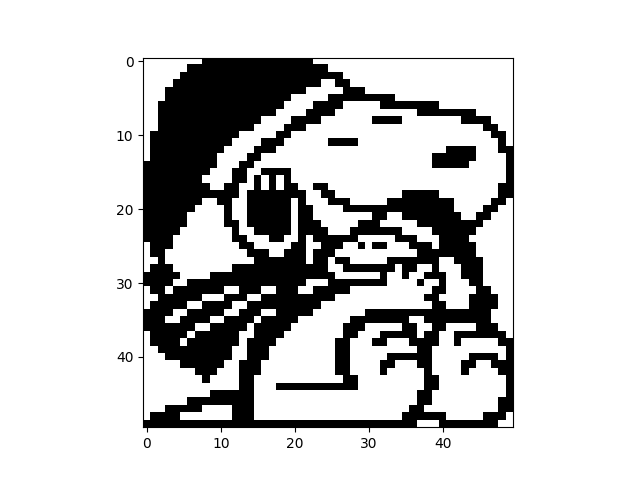
\includegraphics[width=8cm]{../images/dynamique_instance9.png}
  				\caption{Grille de l'instance numéro 9}
  
            \end{minipage}
          \end{figure}



\textbf{Question 9} En appliquant notre programme sur l'instance 11, on observe qu'en dépit de la petite taille de l'instance notre algorithme ne colorie rien. En effet quand une case peut être coloriée à la fois en blanc et en noir notre algorithme ne fais rien. Si la couleur d'une case ne peut être déterminée de manière exacte grace aux contraintes elle ne sera pas coloriée. Ce qui explique pourquoi notre algorithme ne colorie pas correctement l'instance 11.
\\
Une solution à ce problème est d'implémenter un algorithme de backtracking qui une fois la coloration effectuée, observe toutes les cases non coloriées et leur affecte 0 et 1 arbitrairement puis on relance coloration avec la nouvelle grille. On réitère jusqu'à obtenir une grille complète (dans ce cas fin de l'algorithme) ou une grille insolvable. Si le grille ne peut pas être résolue , on retourne jusqu'à l'affectation la plus récente et on prend l'autre couleur. On notera que cette algorithme prend beaucoup plus de temps pour résoudre les grilles, une autre approche est d'utiliser la PLNE.\\
\begin{enumerate}
\item Initialisation : A <- coloration(M) 
\item Tant que la grille n'est pas complète et que le nœud parent n'a pas testé toutes les couleurs:
  \begin{enumerate}
    \item Si coloration(A) != False:\\
      Alors choisir arbitrairement une case incomplète c et lui attribuer une couleur
    \item Si coloration(A) == False:\\
      Alors en retourne à la grille précédente et on attribue l'autre couleur.
    \item  A <- coloration(A)
  \end{enumerate}
\end{enumerate}
\textit{remarque : } Cette algorithme n'a pas été implémenté néenmoins nous allons procéder à une analyse de complexité pire cas. Dans le pire des cas, chaque case restante est examinée 2 fois. Soit n le nombre de cases restantes. On a donc $2^n $ itérations, qui appellent toutes la fonction coloration. Cette algorithme est donc de complexité exponentielle.



 	
 	\newpage
 	\section{II. La PLNE à la rescousse}
    \subsection{1 - Modélisation}
    \textbf{Question 10:}\\\\ On veut avoir une contrainte qui force nos cases  à êtres noires si un bloc est posé. De plus si un bloc n'est pas posé sur la case (i,j), il ne faut rien imposer aux $x_{ij}$ . \\
    Par conséquent la condition est: $\sum \limits_{{k=j}}^{j+s_{t}-1} x_{ik} \geq y^{t}_{ij} \times s_{t}  $ c'est à dire : \\
    $\sum \limits_{{k=j}}^{j+s_{t}-1} x_{ik} - y^{t}_{ij} \times s_{t} \geq 0$ \\
    Cette contrainte est bien valide car si $y_{ij}$ vaut 1 alors toutes les cases associées aux bloc doivent être noires. Et si $y_{ij}$ vaut 0, on n'a pas de contrainte. \\
    Avec le même raisonnement on a pour les colonnes: $\sum \limits_{{k=i}}^{i+s_{t}-1} x_{kj} \geq z^{t}_{ij} \times s_{t} $\\
    \textbf{Question 11:}\\\\
    On cherche à exprimer une contrainte qui empêche de poser un bloc t+1 avant que le bloc t soit posé.

    La condition est: $y^{t}_{ij} + \sum \limits_{{k=0}}^{j+s_{t}} y^{t+1}_{ik} \leq 1$\\
    Si $y_{ij}$ vaut 0, la contrainte est toujours vraie . Et si $y_{ij}$ vaut 1, aucun bloc $k$ avec $k > t$ ne peut être posé avant $j+s_t$. \\
    Avec le même raisonnement on a pour les colonnes: $z^{t}_{ij} + \sum \limits_{{k=0}}^{i+s_{t}} z^{t+1}_{kj} \leq 1$
    \newpage
    
    \textbf{Question 12:}\\\\
   
  Min z = $\sum \limits_{{i=0, j=0}}^{N, M}x_{i,j}$ \\\\
  $$	
	s.c\left\{
    \begin{array}{ll}
         \sum \limits_{{k=j}}^{j+s_{t}-1} x_{ik} - y^{t}_{ij} \times s_{t} \geq 0$ | $\forall i \in \lbrace 0, 1, 2,...,N-1\rbrace, \forall t \in \lbrace 1, 2,...,k_{i}\rbrace\\\\
         
        \sum \limits_{{k=i}}^{i+s_{t}-1} x_{kj} - z^{t}_{ij} \times s_{t} \geq 0 $ | $\forall j \in \lbrace 0, 1, 2,...,M-1\rbrace, \forall t \in \lbrace 1, 2,...,k_{j}\rbrace\\\\
        
        y^{t}_{ij} + \sum \limits_{{k=0}}^{j+s_{t}} y^{t+1}_{ik} \leq 1 $ | $\forall i \in \lbrace 0, 1, 2,...,N-1\rbrace, \forall t \in \lbrace 1, 2,...,k_{i}-1\rbrace\\\\
        
        z^{t}_{ij} + \sum \limits_{{k=0}}^{i+s_{t}} z^{t+1}_{kj} \leq 1$ | $\forall j \in \lbrace 0, 1, 2,...,M-1\rbrace, \forall t \in \lbrace 1, 2,...,k_{j}-1\rbrace\\\\
        
        \sum \limits_{{j=0}}^{M-1} y^{t}_{ij} = 1 $ | $\forall i \in \lbrace 0, 1, 2,...,N-1\rbrace, \forall t \in \lbrace 1, 2,...,k_{i}\rbrace\\\\
        
        \sum \limits_{{i=0}}^{N-1} z^{t}_{ij} = 1 $ | $\forall j \in \lbrace 0, 1, 2,...,M-1\rbrace, \forall t \in \lbrace 1, 2,...,k_{j}\rbrace\\\\

%        \sum \limits_{{k=0}}^{\sum \limit_{{n=1}}^{t-1} sn+1} z^{t}_{ik} = 0 $ | $\forall j \in \lbrace 0, 1, 2,...,M-1\rbrace, \forall t \in \lbrace 1, 2,...,k_{j}\rbrace\\\\

%        \sum \limits_{{k=0}}^{N - st - \sum \limit{_{n=l+1}^{ki}} (sn+1)}} z^{t}_{ik} = 0 $ | $\forall j \in \lbrace 0, 1, 2,...,M-1\rbrace, \forall t \in \lbrace 1, 2,...,k_{j}\rbrace\\\\

        
        
        
      x_{ij} \in \lbrace0,1\rbrace$ | $\forall i \in \lbrace 0, 1, 2,...,N-1\rbrace, \forall j \in \lbrace 0, 1, 2,...,M-1\rbrace\\\\
      
      y^{t}_{ij} \in \lbrace0,1\rbrace $ | $\forall i \in \lbrace 0, 1, 2,...,N-1\rbrace, \forall j \in \lbrace 0, 1, 2,...,M-1\rbrace, \forall t \in \lbrace 1, 2,...,k_{i}\rbrace\\\\
      
      z^{t}_{ij} \in \lbrace0,1\rbrace $ | $\forall i \in \lbrace 0, 1, 2,...,N-1\rbrace, \forall j \in \lbrace 0, 1, 2,...,M-1\rbrace, \forall t \in \lbrace 1, 2,...,k_{j}\rbrace\\\\
    \end{array}\\\\
\right.
$$
\\


\subsection{2 - Implantation et tests}
\textbf{Question 13: }\\\\
(N'oublions pas que j commence à 0 et termine à M-1)\\
- Pour une ligne $l_{i}$ le $l^{ieme}$ bloc ne peut commencer avant la case  $(i, \sum \limits_{{n=1}}^{l-1} (s_{n}+1))$ , ni commencer après la case $(i, M - s_{l} - \sum \limits_{{n = l+1}}^{k_{i}}(s_{n}+1))$. \\
- Pour une colonne $l_{j}$ le $l^{jeme}$ bloc ne peut commencer avant la case  $(i, \sum \limits_{{n=1}}^{l-1} (s_{n}+1))$ , ni commencer après la case $(i, N - s_{l} - \sum \limits_{{n = l+1}}^{k_{i}}(s_{n}+1))$. \\
On ajoute bien évidemment ces contraintes dans notre programme linéaire et mettant les $y_{ij}^t$ et $z_{ij}^t$ à 0, pour les i et j ne faisant pas parties de l'intervalle des blocs possibles.
\newpage
\textbf{Question 14: }\\\\
L'implantation du plne résout parfaitement l'instance 11:
\begin{figure}[h]
\centering
  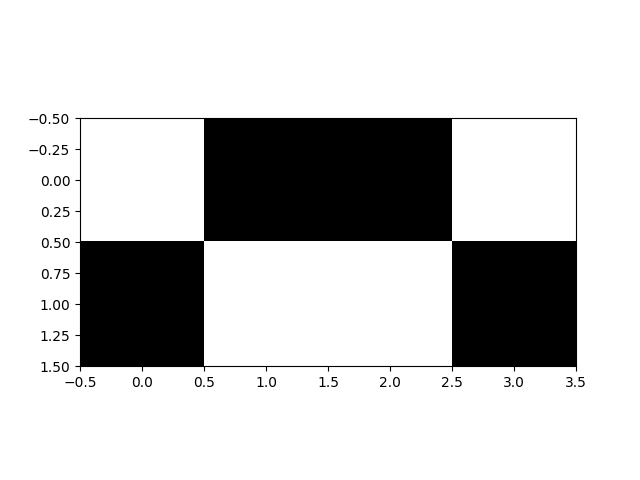
\includegraphics[width=7cm]{../images/plne_instance11.png}
  \caption{Grille de l'instance numero 11}
  \label{fig:plne11}
\end{figure}\\\\
\textbf{Question 15: }

\begin{figure}[h]
  \begin{center}
    \begin{tabular}{|c||c||c||c||c|}
      \hline
      instances & dynamique-time & plne-time & mix-time & nombre de cases \\ 
      \hline
      0 & 0.0004119873046875 & 0.0006170272827148438 & 0.0008900165557861328 & 20 \\ 
      \hline
      1 & 0.0004858970642089844 & 0.0013060569763183594 & 0.0009407997131347656 & 25 \\ 
      \hline
      2 & 0.11206889152526855 & 2.535233974456787 & 0.12527084350585938 & 400 \\ 
      \hline
      3 & 0.08992695808410645 & 0.126816987991333 & 0.10281085968017578 & 481 \\ 
      \hline
      4 & 0.1614398956298828 & 9.870957851409912 & 0.19457793235778809 & 625 \\ 
      \hline
      5 & 0.19578003883361816 & 2.034217119216919 & 0.20783019065856934 & 675 \\ 
      \hline
      6 & 0.5122568607330322 & 351.21364879608154 & 0.5453379154205322 & 900 \\ 
      \hline
      7 & 0.3045821189880371 & 0.4993908405303955 & 0.32914304733276367 & 1054 \\ 
      \hline
      8 & 0.44316697120666504 & 0.8764519691467285 & 0.498075008392334 & 1400 \\ 
      \hline
      9 & 5.620426177978516 & timeout & 5.995676279067993 & 2500 \\ 
      \hline
      10 & 9.328194856643677 & timeout & 10.79225778579712 & 9801 \\ 
      \hline
      11 & 0.0003771781921386719 & 0.0005419254302978516 & 0.0009791851043701172 & 8 \\ 
      \hline
      12 & 0.8796999454498291 & 162.9039990901947 & 1.081050157546997 & 924 \\ 
      \hline
      13 & 1.0365591049194336 & 2.343104124069214 & 1.3090941905975342 & 2025 \\ 
      \hline
      14 & 0.772252082824707 & 0.7354490756988525 & 0.824674129486084 & 1140 \\ 
      \hline
      15 & 0.28334784507751465 & 18.160336017608643 & 7.860313892364502 & 900 \\ 
      \hline
      16 & 0.7040119171142578 & timeout & 1650.8602929115295 & 1750 \\ 
\hline
    \end{tabular}

\caption{Comparaison des temps pour les 2 méthodes}
  \end{center}
  On remarque que la programmation dynamique est la methode la plus rapide mais elle n'est pas capable de résoudre completement les instances a partir de 11. De plus le temps de calcul pour la PLNE semble plus dépendre des contraintes sur les lignes et les colonnes que du nombre de cases. Par exemple elle prend 162 secondes pour résoudre l'instance 12 de 924 cases alors qu'elle résoud l'instance 13 de 2025 cases en 2 secondes ! \\
  Finalement la methode mix qui consiste à initialiser la grille avec la programmation dynamique et à appliquer la PLNE est nettement plus rapide que la PLNE classique.
\end{figure}



\begin{figure}[h]
  \centering
  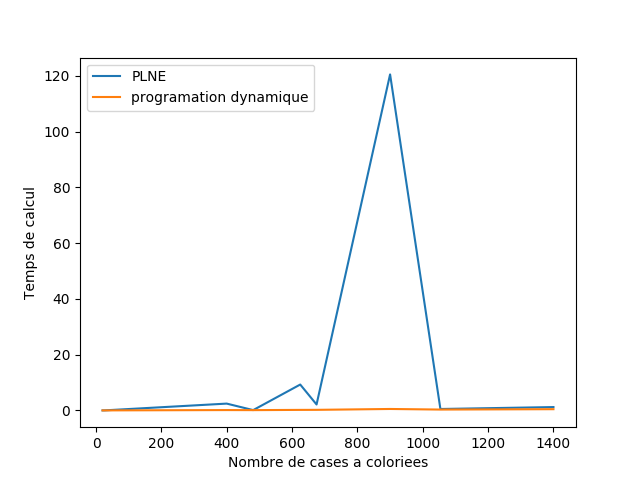
\includegraphics[width=0.75\linewidth]{../images/comparaison.png}
  \caption{Comparaison des deux méthodes sur les 8 premières instances}
  \label{fig:graphes-comparaison}
\end{figure}

\begin{figure}[h]
 Dans la figure 0.6, le gris correspond aux cases blanches, le noir aux cases noires et le blanc aux cases non déterminées\\\\
\begin{minipage}[c]{.45\linewidth}
  \centering
    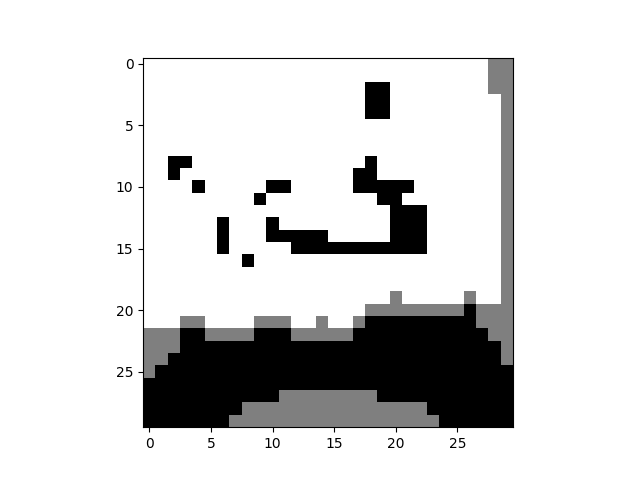
\includegraphics[width = 7cm]{../images/dynamique_instance15.png}
    \caption{Images de l'instance 15 avec la programmation dynamique}
    \label{fig:dynamique15}
\end{minipage}\hfill
\begin{minipage}[c]{.45\linewidth}
    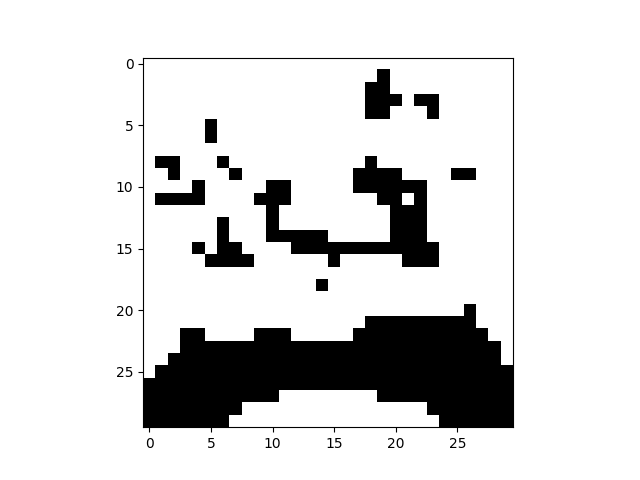
\includegraphics[width = 7cm]{../images/plne_instance15.png}
    \caption{Image de l'instance 15 avec la PLNE}
    \label{fig:plne15}
\end{minipage}
\end{figure}

\begin{figure}[h]
  \section{III. Pour aller plus loin}
  \textbf{Analyse de complixté:} On étudie la complexité pire cas de l'algorithme de programmation dynamique de la partie 1.
  Soient I et J le nombre de contraintes sur les lignes et colonnes.
  La fonction T(j,l) va calculer toutes les combinaisons de cases et séquences  pour les lignes et les colonnes ce qui ce fait en $O(I \mult N + J \mult M)$ si l'on considère la version itérative. \\
  L'algorithme de coloration est basé sur une boucle while.
  Dans le pire des cas on a une boucle pour chaque case de la grille. Donc la complexité de l'algorithme est $O(N\mult M\mlut (I \mult N + J \mult M))$.\\
  La complexité expérimentale semble bien plus faible.On fait l'hypothèse que nous avons une fonction polynomiale de la forme $f(x) = \lambda x^p$ avec $\lambda$ et $p$ appartenant à $\mathbb{R}$. De ce fait en passant au log on obtient : $log(f(x)) = log(\lambda) + p \times log(x)$ avec $log(\lambda)$ une constante. De ce fait, en tracant $log(f(x))$ en fonction de $log(x)$ et en calculant la pente on obtient $p$, c'est à dire la puissance de notre polynome.
  En procédant ainsi nous trouvons p=0.562258487574. \\
  
En implémentant la méthode qui consiste à commencer par la programmation dynamique puis la PLNE sur les cases non déterminées nous obtenons des meilleurs temps comme on peut le voir ci-dessous:\\\\
\begin{center}
\begin{tabular}{|c||c||c|}
\hline
instances & plne-time & mix-time \\ 
\hline
11 & 0.000541925430298 & 0.00097918510437 \\ 
\hline
12 & 162.90399909 & 1.08105015755 \\ 
\hline
13 & 2.34310412407 & 1.3090941906 \\ 
\hline
14 & 0.735449075699 & 0.824674129486 \\ 
\hline
15 & 18.1603360176 & 7.86031389236 \\ 
\hline
16 & timeout & 1650.86029291 \\ 
\hline
\end{tabular}
\end{center}

\caption{Comparaison des temps entre la plne pure et avec une initialisation avec la programmation dynamique(mix)}
\\
\textbf{Conclusion : }La methode de résolution la plus rapide est la programmation dynamique. Mais elle n'est pas capable de résoudre certain types de grilles plus difficiles ou il y a un choix de couleur arbitraire à faire pour la résoudre. La PLNE permet de résoudre ces instances mais c'est une methode lente car nous utilisons des variables binaires donc gurobi fait un branch and boud pour trouver la solution optimale. Par conséquent c'est un problème np-complet. On peut néenmoins améliorer le temps de résolution en calculant une grille partielle à l'aide de la programation dynamique et en appliquant la PLNE sur cette grille.
\end{figure}

        
\end{document}
